\documentclass[11pt,a4paper]{article}

%---------------------------------------------------------
%	Aditional Packages
%--------------------------------------------------------
\usepackage{textpos}
\usepackage{subcaption} % To have multiple plots side by side
\usepackage{float}
\usepackage{url} % enable clickable URLs
\usepackage{listings} % to have code blocks in your document
\usepackage{xcolor}
\usepackage{doi}
\usepackage{microtype}
\usepackage{booktabs}
\usepackage{nicefrac} % creates a fraction that is nicer when used in text \nicefrac{1}{2}

% Define some colors for code 
\definecolor{codegreen}{rgb}{0,0.6,0}
\definecolor{codegray}{rgb}{0.5,0.5,0.5}
\definecolor{codepurple}{rgb}{0.58,0,0.82}
\definecolor{backcolour}{rgb}{0.95,0.95,0.92}

% Defines codeblock styles
\lstdefinestyle{mystyle}{
    backgroundcolor=\color{backcolour},   
    commentstyle=\color{codegreen},
    keywordstyle=\color{magenta},
    numberstyle=\tiny\color{codegray},
    stringstyle=\color{codepurple},
    basicstyle=\ttfamily\footnotesize,
    breakatwhitespace=false,         
    breaklines=true,                 
    captionpos=b,                    
    keepspaces=true,                 
    numbers=left,                    
    numbersep=5pt,                  
    showspaces=false,                
    showstringspaces=false,
    showtabs=false,                  
    tabsize=2
}

% Set the maximum depth sections are counted to and shown in the TOC
\setcounter{secnumdepth}{3} % depth of counting
\setcounter{tocdepth}{3} % depth that toc will show 

% new paragraph style with new line
\newcommand{\myparagraph}[1]{\paragraph{#1}\mbox{}\\}


\lstset{style=mystyle}
\renewcommand{\lstlistingname}{Configuration}% Listing -> Configuration

% Toogle between the two to hide or show images
% \usepackage[draft]{graphicx}
\usepackage{graphicx}
\usepackage[utf8]{inputenc} 
\usepackage{upgreek}
\usepackage{titlesec}
\usepackage{physics} % adds easy derivatives etc. 
%\AtBeginDocument{\RenewCommandCopy\qty\SI} % dont know why
\usepackage{amssymb} % more symbols
\usepackage{amsmath} %enables align environment
\usepackage{multirow}


% \usepackage[showframe]{geometry} % Shows margins in pdf if you want to know what's going on
\usepackage{geometry}
\geometry{
    %a4paper,
	left=40mm,
    % right=20mm,
	top=35mm,
    }

% Use biblatex
\usepackage[backend=biber,
natbib=true,
maxcitenames = 2,
maxbibnames = 5,
minbibnames = 4, 
sorting=none]{biblatex}

\usepackage{csquotes}

\addbibresource{references.bib}
\setlength\bibitemsep{1.5\itemsep}


% --------------------------------------------------------
% CUSTOM STUFF:
% \usepackage[textsize=tiny]{todonotes}
% \setlength{\marginparwidth}{2cm}
\usepackage{bm}
%---------------------------------------------------------
\usepackage{hyperref} % enable clickable links to sections, figures, etc. 
\PassOptionsToPackage{unicode}{hyperref}
\PassOptionsToPackage{naturalnames}{hyperref}

% Remove the coloured border around autoref links
\hypersetup{%
pdfborder = {0 0 0}
}



\begin{document}	
\pagestyle{empty}

%---------------------------------------------------------
%	Titlepage
%---------------------------------------------------------

\begin{center}
    \vspace*{1cm}
    \LARGE \bf{Structure recognition with graph neural networks} \\

    \vspace*{2cm}
    \large \bf{An intermediate report for the course "Advanced Projects in Computational Physics 2"}


    \vspace{4cm}
    
    \vspace{1.2cm}
            From\\
            {\bf Stephen Weybrecht} \\
            \today

    \vspace*{6 cm}
    Tutor: Jonas Buba \\
    Supervisor: Prof. Dr. Schmiedeberg
    \vspace*{1 cm}

\end{center}
\clearpage
%---------------------------------------------------------
%	Table of Contents
%---------------------------------------------------------
% Generate
\newgeometry{
    %a4paper,
	%left=20mm,
    right=40mm,
	top=35mm,
    } 
\tableofcontents
\restoregeometry
\clearpage
\mbox{}

\pagenumbering{arabic}
\setcounter{page}{1}
 
%---------------------------------------------------------
%	Report
%---------------------------------------------------------

\section{Theoretical introduction}
\label{sec:Theoretical introduction}

\subsection{Bravais lattices}
\label{ssec:Bravais lattices}
In the first part of the project, our task was to deal with crystal lattices in 2 and 3 dimensions. 
For the following discussion an introduction of the terms "crystal", "basis" and "Bravais lattice" is therefore needed. \\

Following the discussion of \cite{kittelChapter1Crystal2005} an ideal crystal is a periodic, infinite arrangement of atoms in a solid. 
These atoms are arranged in blocks, a so called basis, in a regularly spaced grid, the lattice. 
In other words the lattice represents a schema after which individual atoms or groups of atoms (the basis) are arranged to form the crystal. 
A lattice in $d$ dimensions can be defined by a set of $d$ translation vectors. 
THe superposition of integer multiples of these vectors then makes up the lattice. 
In principle the length and direction of these vectors can be arbitrary. 
In this case the lattice would generally not map into itself under translations and rotations -- the lattice is called oblique. 
There are however special sets of translation vectors which form lattices of high symmetry. 
These fundamental lattices are called the Bravais lattices. 
For $d=2$ there are 5 (4 special and one oblique) Bravais lattices, while for $d=3$ there are 14 (13 special cases and one oblique, so called triclinic lattice). 
These are depicted in \autoref{fig:bravais2D} and \autoref{fig:bravais3D} respectively. 

\begin{figure}[htbp]
    \centering
    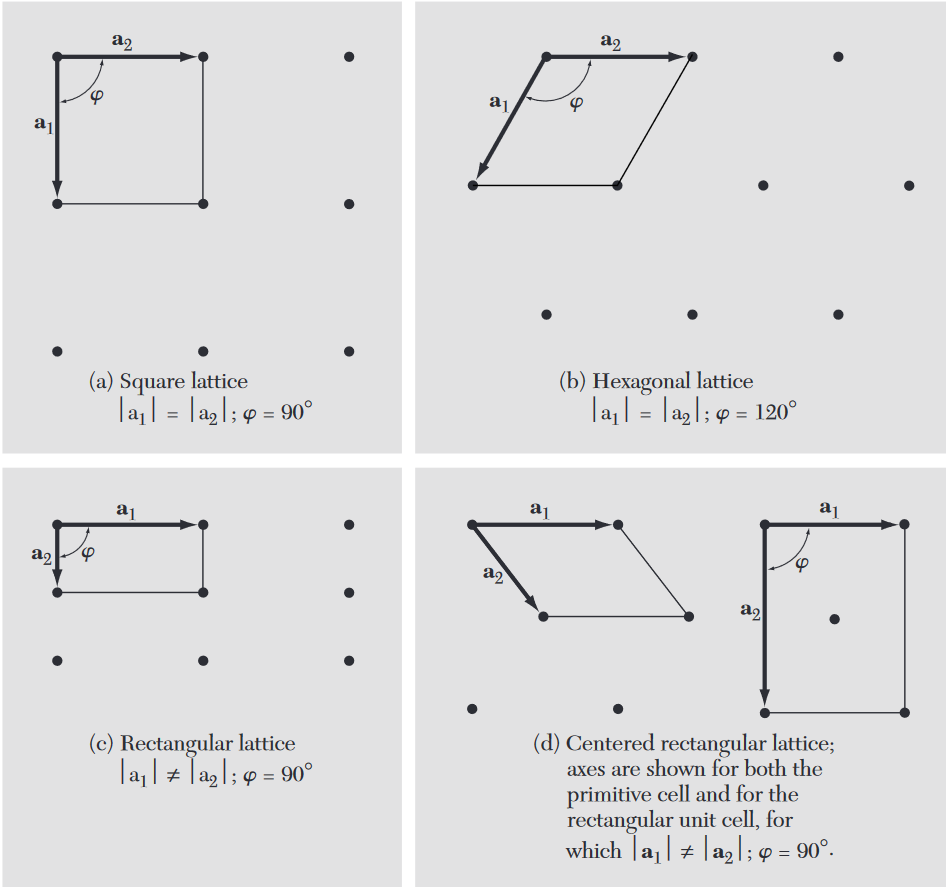
\includegraphics[width=0.6\textwidth]{images/Kittel_7.png}
    \caption{The five Bravais lattices for 2 dimensions. The graphic also illustrates the length of the translation vectors $\bm{a}_i$ and the angle between them in order to make up the corresponding lattice. Taken from \cite[Fig. 7]{kittelChapter1Crystal2005}.}
    \label{fig:bravais2D}
\end{figure}

\begin{figure}[htbp]
    \centering
    \includegraphics[width=0.7\textwidth]{images/Kittel_14.png}
    \caption{The 14 Bravais lattices for the $d=3$ case. 
    One further classifies these lattices into seven types of cells: Cubic ($a{=}b{=}c$, $\alpha {=} \beta {=} \gamma{=}90^\circ$), Tetragonal ($a{=}b {\neq} c$, $\alpha {=} \beta {=} \gamma{=}90^\circ$), Orthorhombic ($\alpha {=} \beta {=} \gamma{=} 90^\circ$), Monoclinic ($\alpha {=} \beta{=}90^\circ {\neq} \gamma$), Triclinic, Triagonal ($a{=}b{=}c$, $\alpha {=} \beta {=} \gamma <120^\circ {\neq} 90^\circ$), Hexagonal ($a{=}b{\neq} c$, $\alpha {=} \beta{=} 90^\circ, \gamma{=} 120^\circ$). 
    Note that in the prior notation $a$, $b$ and $c$ denote the lenghts of the translation vectors, $\alpha$, $\beta$, $\gamma$ the angles between them and omitted length or angle relations mean they can be arbitrary. 
    These groups are again subclassified based on their lattice structure into simple "P", body-centred "I", base-centred "C", face-centred "F". 
    As mentioned, all lattices are special cases of the general, triclinic case. The graphic is taken from \cite[Fig. 14]{kittelChapter1Crystal1971}}
    \label{fig:bravais3D}
\end{figure}

\subsection{Graph neural networks}
\label{ssec:Graph neural networks}
The lattices as discussed in the prior section are a collection of atoms linked by bonds and can therefore be suitably represented by a graph, consisting of nodes and edges. 
If we want to apply machine learning to crystal lattices, we therefore need models that are well suited for data organized in a graph-like manner. 
What follows is a basic introduction to such networks, specificially graph concolutional neural networks (GCNs). \\

GCNs take inspiration in the already well-established convolutional neural networks in which a typical layer consits of a trainable kernel that can be applied on ordered, grid-like training data of arbitrary size and shape (e.g. images) \cite{khemaniReviewGraphNeural2024}. 
GCNs represent a generalisation of this concept onto unordered nodes with a variable number of neighbours. 
Each GCN-layer uses so called message passing in order to update the node state $h^{(t)}_u$ of a time $t$ to the next step $h^{(t+1)}_u$ as shown in \autoref{eq:messagepassing} \cite[eq. 4.1]{khemaniReviewGraphNeural2024}.
\begin{equation}
    h^{(t+1)}_u = UPDATE^{(t)}\left(h^{(t)}_u, AGGREGATE^{(t)}\left(\left\{h^{(t)}_v, \forall v \in N(u)\right\}\right)\right)
    \label{eq:messagepassing}
\end{equation}
In the above equation $UPDATE^{(t)}$ and $AGGREGATE^{(t)}$ could be any differentiable functions i.e. also neural networks, and $N(u)$ denotes the neighbourhood of $u$ meaning all directly connected nodes in the graph. 
This equation implies the following update schema that is also depicted in \autoref{fig:messagepasisng}: \\
The starting point is a graph, consisting of nodes with feature vectors and connections, that could also have features. 
For each node, messages from neighbouring nodes are aggregated to a single message by taking a weighted mean of the neighbouring nodes feature vectors. 
This operation can also be weighted by use of edge features. 
This message is then passed to a nonlinear update function (e.g. ReLU), that updates the node in question for the next timestep. 
After the update is completed, further operations can be performed depending on the wanted classification scheme. 
In the following graph classification is used, which means all feature vectors are pooled in a last step, in order to get a single quantity that is descriptive of the entire graph \cite{khemaniReviewGraphNeural2024}.
\begin{figure}[htbp]
    \centering
    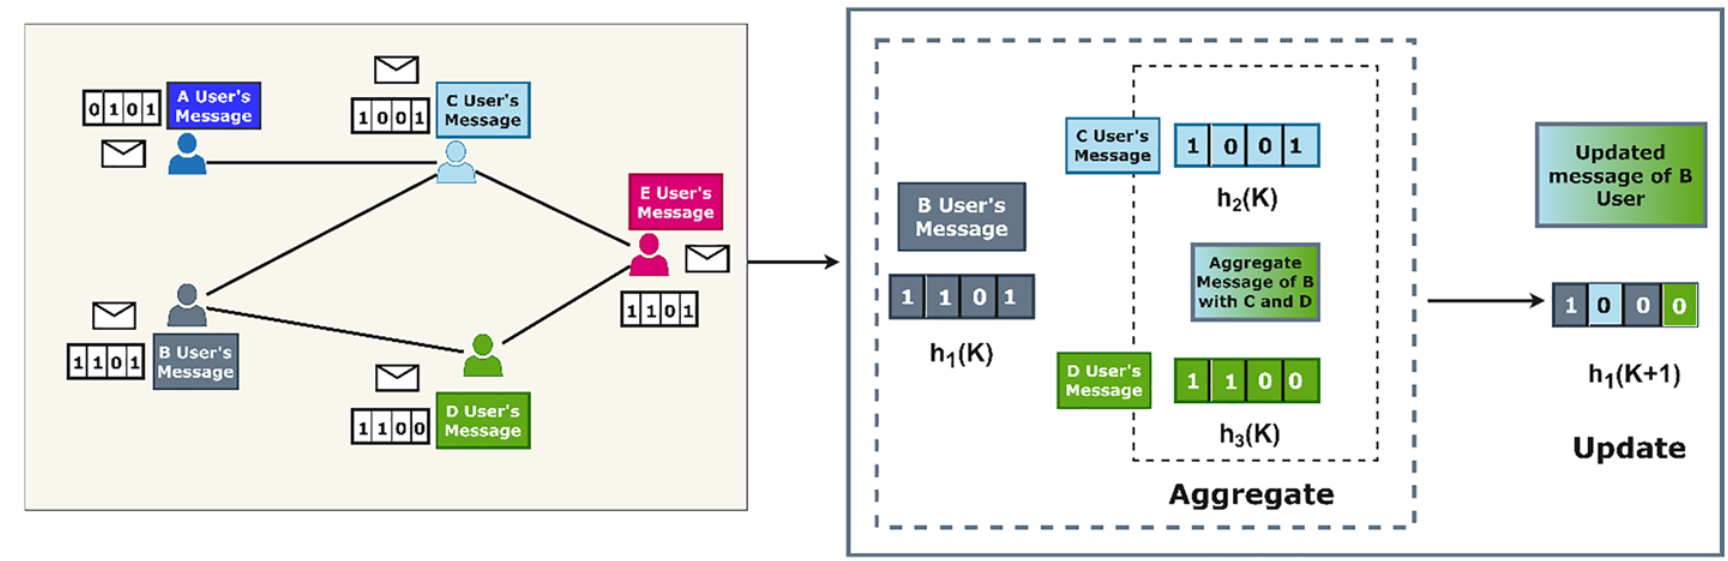
\includegraphics[width=0.9\textwidth]{images/khemani7.png}
    \caption{A graphic representation of the update schema for message passing graph neural networks. Taken from \cite[Fig. 7]{khemaniReviewGraphNeural2024}.}
    \label{fig:messagepasisng}
\end{figure}

\section{Results so far}
\label{sec:Results so far}

\section{Plans for the future}
\label{sec:Plans for the future}


%---------------------------------------------------------
%	Bibliography
%---------------------------------------------------------

\newgeometry{
	%a4paper,
	left=40mm,
    % right=20mm,
	top=35mm,
}
\renewcommand\refname{Bibliography}
% \printbibliography
\printbibliography[
heading=bibintoc,
title={Bibliography}
]


\end{document}

